%% ----------------------------------------------------------------
%% Object Detection.tex
%% ---------------------------------------------------------------- 
\chapter{Object Detection} \label{Chapter:ObjectDetection}

Object detection is the natural extension to the image classification problem. In image classification, for each sample there is a single output denoting the class of the sample. In mathematical notation for each sample $X$, the model $\phi$, $\phi(X)$, gives as output an $N-$vector $P_x=(p_1,p_2,...,p_N)$\footnote{$\sum^N_i p_i=1$}, where each element indicates the probability of the sample belonging in class $n_i \in N$. Object detection pushes this task a bit further by classifying and localising an instance in the image, instead of simply making a prediction. Therefore, for each sample query the output includes the predicted class and a set of coordinates that define a bounding box around the object; there could be more than one predictions for a single image. Despite that traditional object detection includes class prediction and a rectangle bounding box around the class, the vision community evolved object detection to image segmentation and instance segmentation. In image segmentation, the model is called to classify images pixel-wise where each pixel represents a class, while in instance segmentation the model segments the observed classes in objects and background. While object detection had started years prior deep learning's revolution, the most significant and robust algorithms have a deep learning approach. In general, deep learning based object detectors are divided in \textbf{\textit{double stage detectors}} and \textbf{\textit{single stage detectors}}. An overview of these methods will be given in the next sections along with the most significant models. 

\begin{figure}[!htb]
  \centering
  \subfigure[Classification.]{
    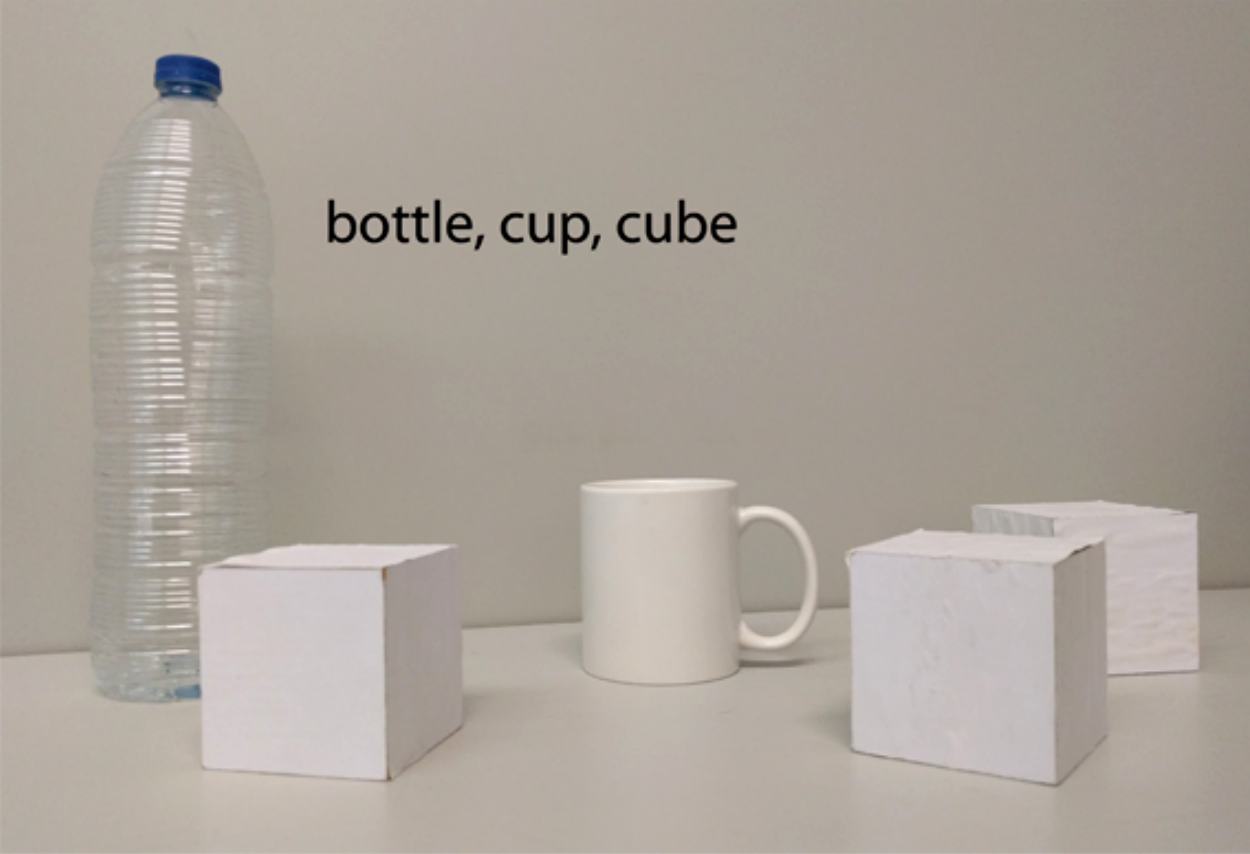
\includegraphics[width=4cm]{images/ch2/fig1_1.png}
    \label{fig1_1}
  }
  \subfigure[Detection (classification + localisation).]{
    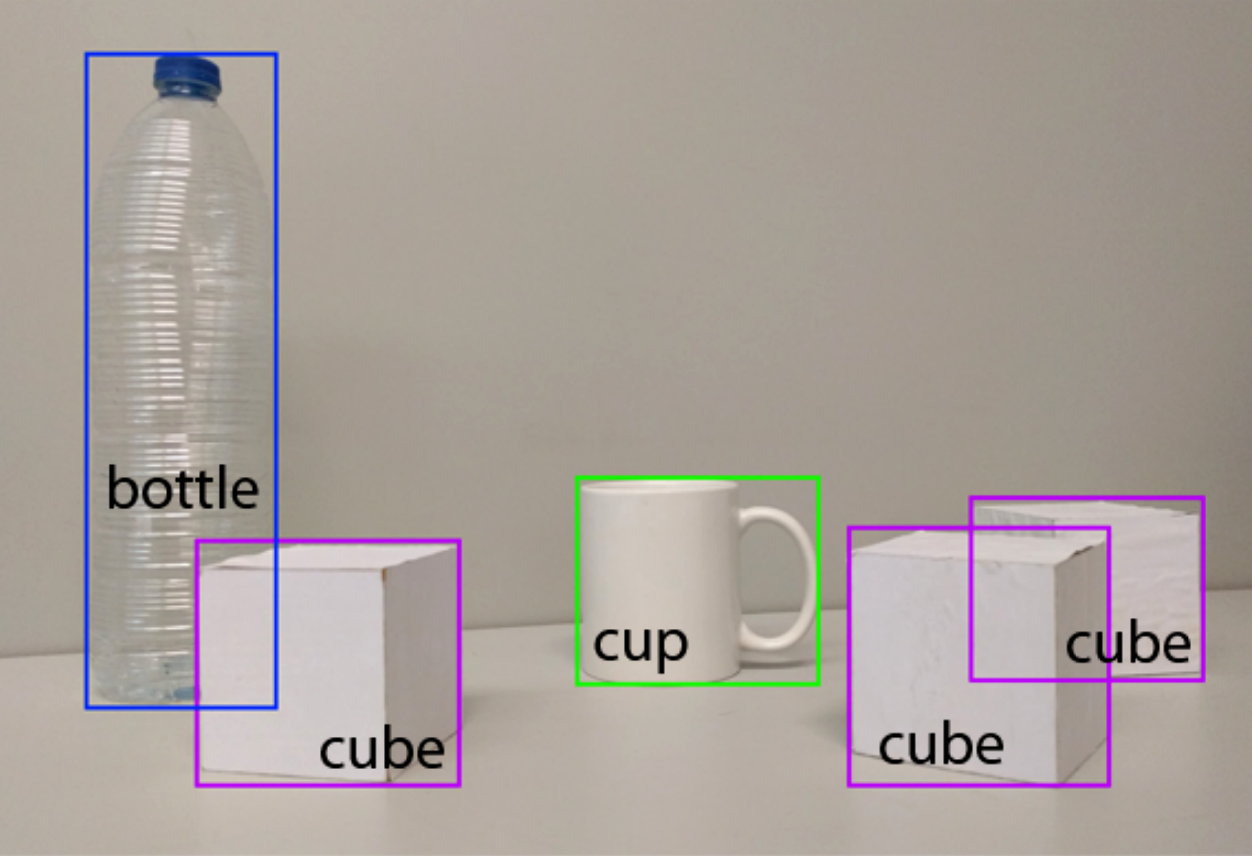
\includegraphics[width=4cm]{images/ch2/fig1_2.png}
    \label{fig1_2}
  }
  
    \subfigure[Image segmentation.]{
    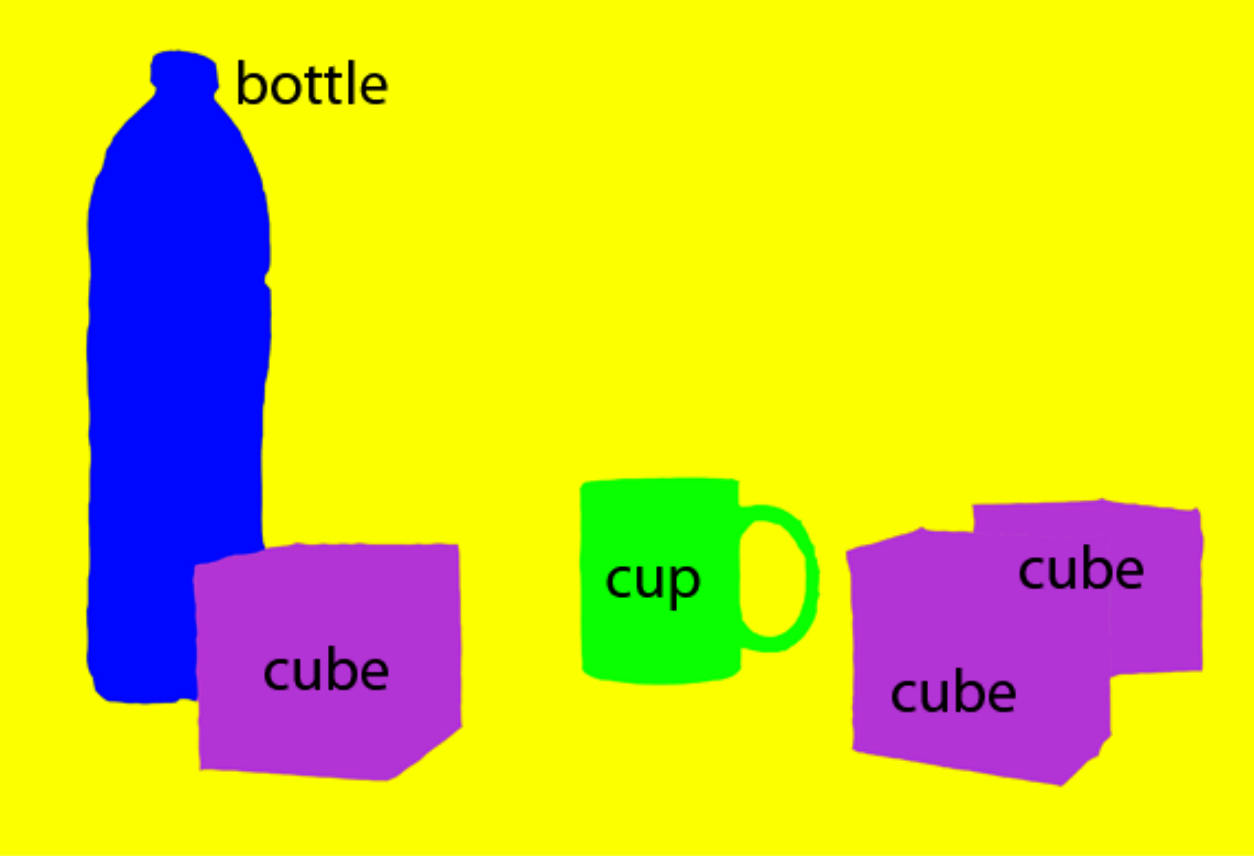
\includegraphics[width=4cm]{images/ch2/fig1_3.png}
    \label{fig1_3}
  }
    \subfigure[Instance segmentation.]{
    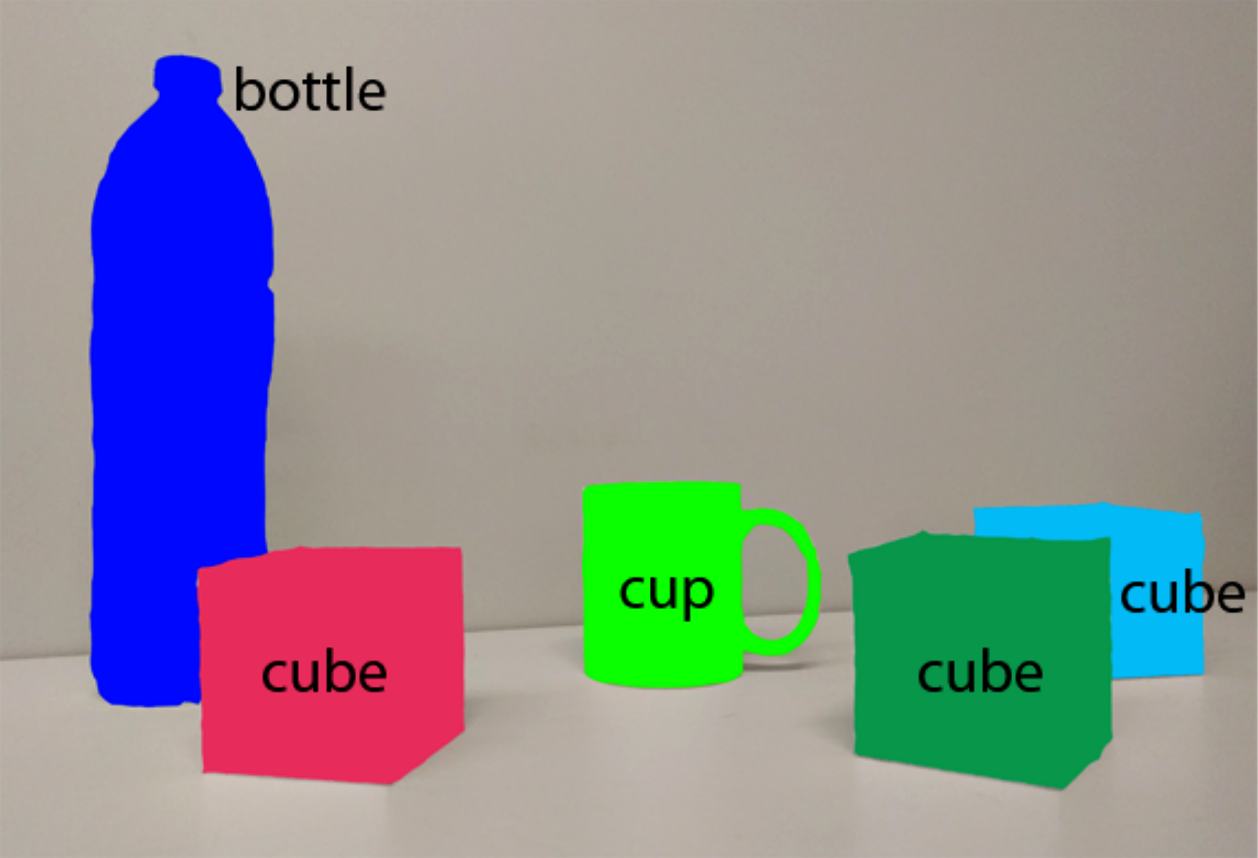
\includegraphics[width=4cm]{images/ch2/fig1_4.png}
    \label{fig1_4}
  }
  \caption{Each task provides semantically richer information (Reproduced from \cite{garcia1704review}).}
  \label{fig1}
\end{figure}

\section{Double-Stage Detectors}

The detection process in double stage or \textbf{\textit{region proposal based detectors}}, can be split in two parts. The first part generates class-agnostic regions of interest (RoIs) with a bounding box around them and the second part predicts the class of each proposed RoI and refines the bounding box around it. It's worth presenting a very popular method in double stage detectors called "R-CNN: Regions with CNN features" (\cite{girshick2014rich}) and its successors Fast R-CNN (\cite{girshick2015fast}) and Faster R-CNN (\cite{ren2015faster}) as Faster R-CNN still stays in fashion due to its high performance.

\subsection{R-CNN}
Before R-CNN was published, object detection was in stagnation without any significant improvement. R-CNN was the first method, that outperformed the previous state-of-the-art CNN method, OverFeat (\cite{sermanet2013overfeat}), increasing accuracy by a big margin. Specifically, R-CNN achieved a mean average precision (mAP) of 31.4\% on ILSVRC2013 (\cite{deng2009imagenet})dataset, over OverFeat which had the previous best result 24.3\%.

R-CNN consists of three parts. The first part generates 2000 class-agnostic regions of interest using selective search (\cite{uijlings2013selective}) with most of them being negative examples. Each proposed region of interest, acts as a potential detection defined by its bounding box. Then, these proposals are warped to a fixed size in order to match architecture's input size criteria. 
The second part is a CNN, pre-trained on the ImageNet dataset (fine-tuned on the new data), and acts as a feature extractor from its last fully connected layer.
The 4096-dimensional extracted features from each RoI, are then classified by class-specific SVMs (plus background) in the last step. After a detection is scored, class-specific box regressors regress the bounding box offsets resulting in a refined bounding box.

\begin{figure}[!htb]
  \centering
  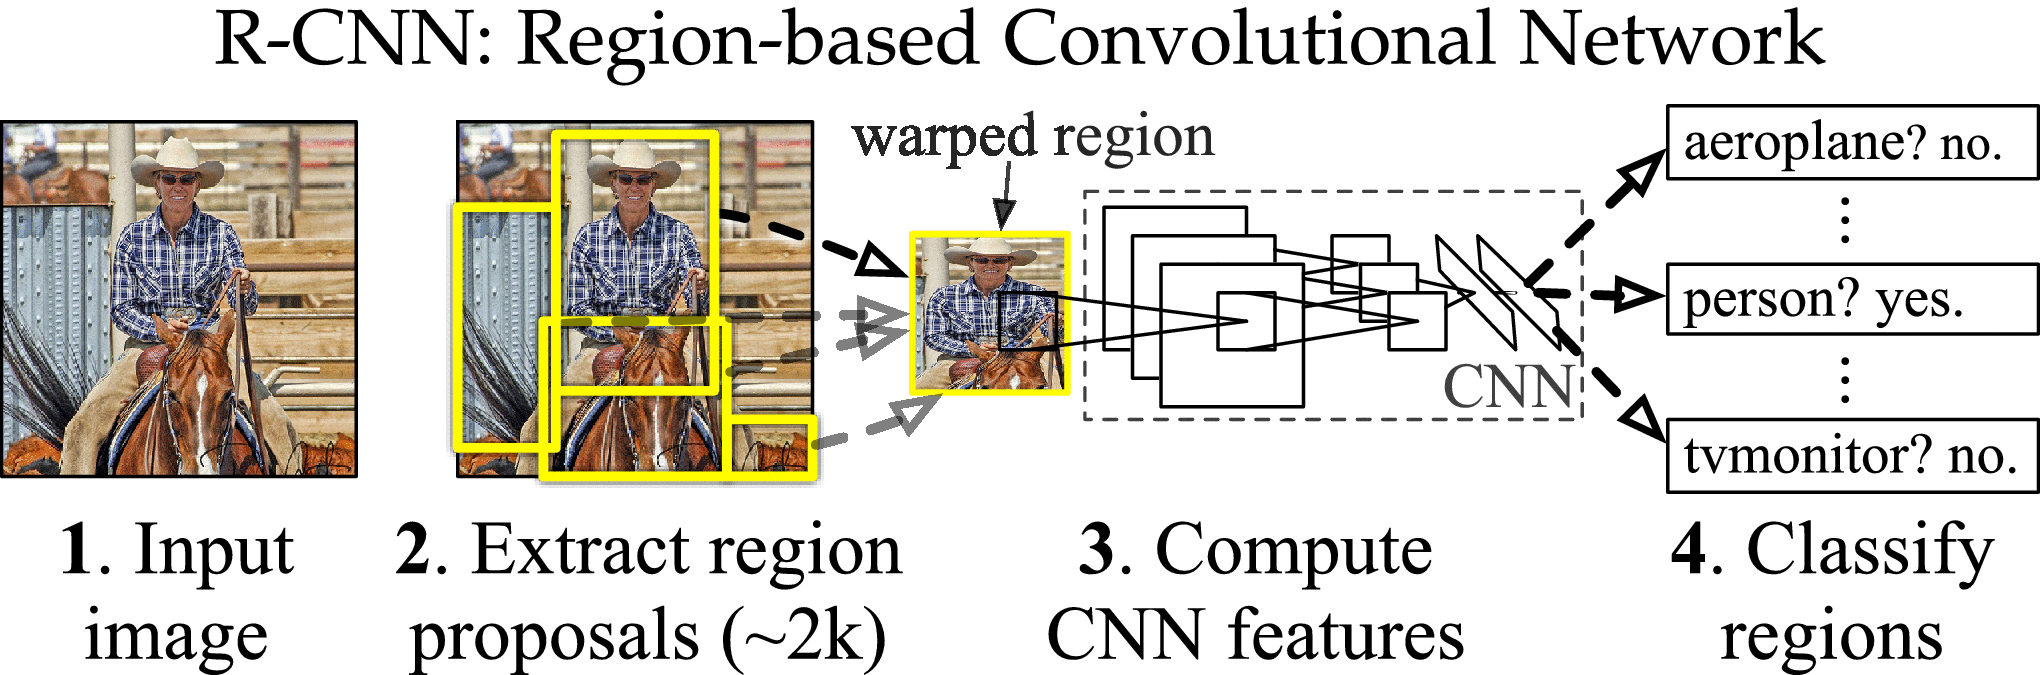
\includegraphics[width=12cm]{images/ch2/fig2.png}
  \caption{R-CNN pipeline as presented in \cite{girshick2014rich}.}
  \label{fig2}
\end{figure}

Although, R-CNN increased performance margin strikingly, has the following notable drawbacks:

\begin{itemize}
  \item The selective search is a heuristic based algorithm, thus it is unable to learn anything during the training procedure. 
  \item Training time takes a vast amount of time and space considering that for each image 2000 proposals have to be fed to the network. Since training it is a multi-stage pipeline, extracted features have to be cached on disk before passed to the SVMs and box regressors. Notice that since the majority of samples are negatives, the authors adopted hard negative mining forcing the model to focus on hard examples (\cite{felzenszwalb2009object}) in order to accelerate convergence.
  \item It is not suitable for real time applications as it has a GPU test rate of  47 seconds/images, when OverFeat was 9x times faster (\cite{girshick2015fast}). 
\end{itemize}

\subsection{Fast-RCNN}
Fast-RCNN was introduced as the improved version of R-CNN, where the multi-stage network was replaced by a single-stage pipeline able to be trained in one stage.

\begin{figure}[!htb]
  \centering
  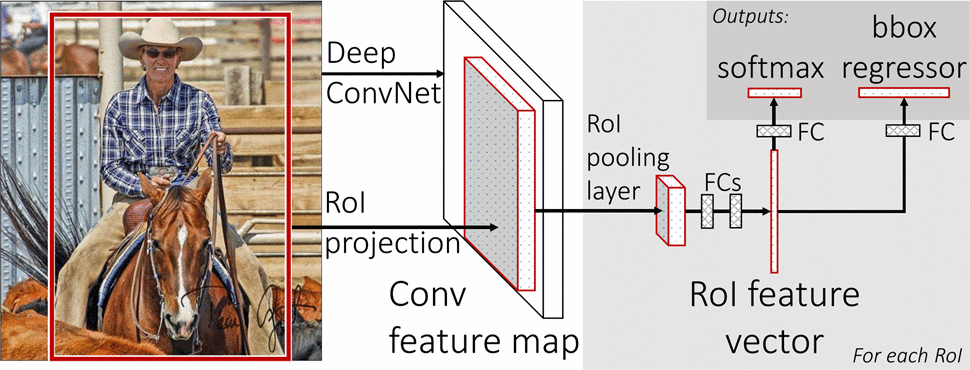
\includegraphics[width=12cm, height=3cm]{images/ch2/fig3.png}
  \caption{Fast R-CNN pipeline as presented in \cite{girshick2015fast}.}
  \label{fig3}
\end{figure}

To achieve this, Faster R-CNN adopted a method from SPPnet (\cite{he2015spatial}) called RoI pooling. R-CNN was handling proposals by warping them into a fixed size and feeding them into the network one by one. On the contrary, SPPnet and Faster-RCNN compute varying size feature maps of the entire image instead of warped region proposals. Each feature map contains RoI information in a four-tuple $(r,c,w,h)$, where $r, c:$ top-left corner and $w, h:$ width and height. Fixed size RoI feature vectors are pooled from variable size feature maps through RoI pooling. Figure \ref{fig4} presents how RoI pooling extracts fixed length feature vectors from feature maps with variable sizes. Moreover, the SVMs and the box regressors are replaced by a joint sibling layer. One layer produces the softmax probability over K + 1 background classes, while the other predicts offsets for the refined bounding boxes. Figure \ref{fig3} illustrates an overview of the model. 

\begin{figure}[!htb]
  \centering
  \subfigure[Feature map with 2 RoIs.]{
    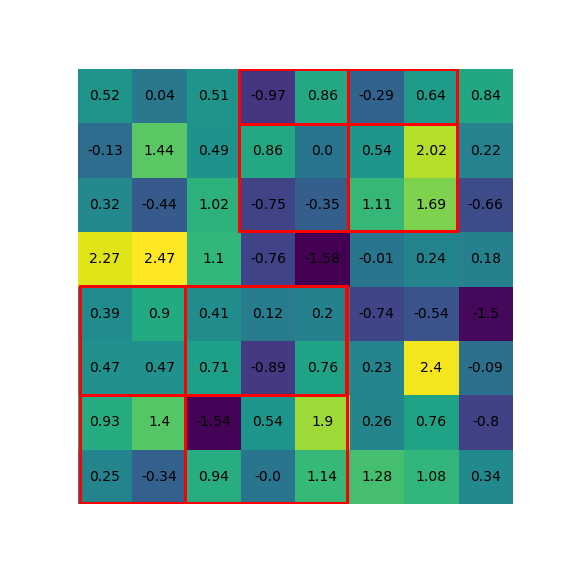
\includegraphics[width=6cm]{images/ch2/fig4_1.png}
    \label{fig1_1}
  }
  \subfigure[RoIs after RoI pooling.]{
    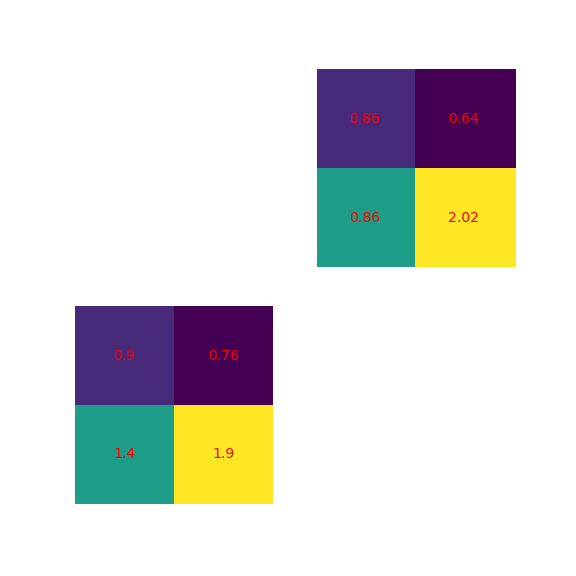
\includegraphics[width=6cm]{images/ch2/fig4_2.png}
    \label{fig1_2}
  }
  \caption{In order to extract vectors of fixed length, different sized proposed RoIs are divided in a fixed number of bins appropriately.}
  \label{fig4}
\end{figure}

By feeding the entire image into the network instead of $\sim$2k proposals one by one, the network avoids redundant computations since a lot of proposals are overlapping each other, hence it is more efficient than its predecessor both in terms of time and memory. Specifically, it is 10x faster than R-CNN in training time and 213x in testing. Furthermore, a joint loss $\mathcal{L}=\mathcal{L}_{cls}+\mathcal{L}_{reg}$ from the softmax and the regression layers optimises the network.

\subsection{Faster-RCNN}
After the replacement of the SVMs with softmax functions, Fast-RCNN was the state-of-the-art object detector, based almost entirely on convolutional neural networks. Its major disadvantage was that the region proposal method, selective search, was not a learning method but a heuristic approach. Soon, this was fixed by the introduction of Faster-RCNN (\cite{ren2015faster}) which entirely dismissed selective search and replaced it with a trainable region proposal network (RPN). RPN, is a CNN where the network's output is attached to a class predictor and a box regressor. The class predictor has only two classes (object, not object), thus the networks is trained to propose regions of interest by their "\textit{objectness}". The rest of the network is adopted by the Fast-RCNN pipeline. Faster R-CNN is classified in the double-stage detectors even if the region proposal method is not decoupled, anymore, from the main pipeline, due to it's 4-step alternate training:
 
\begin{enumerate}
  \item RPN is initialised with the ImageNet weights and fine-tuned for the region proposal task.
  \item The detector (Fast-RCNN) is initialised with the ImageNet weights and fine-tuned for the detection task, with the proposed regions of interest from the RPN (the two models do not share any convolutional layers).
  \item The detector is used to initialise the RPN training, with keeping constant weights coming from shared layers and updating only weights from unique layers. At this point the two models share convolutional layers.
  \item Keeping constant weights from common convolutional layers, detector's unique layers are fine-tuned. 
\end{enumerate}

Faster R-CNN's greatest success is that it consists of a single-stage end-to-end trainable network, entirely based on CNNs with an inference time of 5 FPS.


\section{Single-Stage Detectors}
The downside of double-stage detectors is that training time is split in two separate parts, the region proposal and the detection part, hindering real-time detection. Single-stage detectors or \textbf{\textit{regression/classification based detectors}} have the advantage of being really fast. The main reason is that instead of making class predictions and refining bounding boxes on already proposed regions, apply global rules in every pixel inferring relevant detections without intermediate mechanisms. In this category, the most important algorithms are the Single Shot MultiBox Detector (SSD, \cite{liu2016ssd}), the YOLO model (\cite{redmon2016you}) and RetinaNet (\cite{lin2017focal}) and will synopsised in the next pages.
 
 \subsection{YOLO}
 
\subsection{SSD}

\subsection{RetinaNet}

\section{The Accuracy/Speed Trade-Off}

\section{Evaluation Metrics}

\dots